\chapter{Life After Selling Your Company For \$1 Billion}

This chapter begins as a street-level curiosity about income and quickly turns into a more serious lecture on scale, constraint, and judgment. Glenn Boyd does not give us a formal theory of wealth; he gives us something more useful for note-taking: a sequence of operating heuristics about skill, market size, attention, privacy, security, startup selection, and recession deployment. The mathematics here is light and schematic, but it is not absent. It appears in timescales, capital constraints, changing input costs, and the causal chains by which one technological condition leads to another.

\begin{remark}
This is a conversational lecture rather than a blackboard derivation. Whenever we write an equation below, we are compressing a spoken constraint or causal claim into a cleaner form; we are not pretending that the interview itself presented formal notation.
\end{remark}

\section{Exit, Retirement, and the Return to Work}

The opening surprise is numerical. Glenn says that the company he founded in the original dot-com era was later sold in a merger for roughly \$1.03 billion. That figure is important, but it is not the chapter's endpoint. The real narrative motion begins only after the number has been spoken: retirement, a yacht, years of travel, time with children, then boredom, and finally a return to startup work.

\begin{equation}
V_{\mathrm{sale}} \approx 1.03\times 10^{9}\ \mathrm{USD}.
\end{equation}

The first lesson is immediate. Capital changes the feasible set, but it does not remove the need for purpose, structure, and activity. We are therefore not reading a triumphal story about the moment of exit alone. We are reading a study in what remains after an exit: judgment about what to build, how to spend time, and how to return to work without financial desperation as the primary driver.

\paragraph{Claim.} Liquidity solves one class of problems and leaves another class untouched.

\paragraph{Mechanism.} Once the immediate scarcity problem has been solved, other constraints become visible: boredom, the need for meaningful work, and the persistent requirement to allocate attention well.

This is why the interview does not stay long at the headline number. It pivots backward and asks what kind of formation produced the person who could build such a company in the first place.

\section{From Scarcity to Company Formation}

The biographical sequence matters because it establishes not just hardship, but the way hardship was converted into technical competence. Glenn begins in poverty: roofing houses with his father in Texas, washing dishes to help his mother pay rent, then moving to Southern California as a teenager. There he becomes a busboy, begins dabbling in software and computers around 1980, teaches himself to program, and discovers that the skill is not merely interesting but commercially usable.

\paragraph{Anecdote.} By his own account, he is working full time at sixteen, drops out of high school, and starts getting contracting work because he is already good enough to be paid.

\paragraph{Claim.} Before outside capital enters, technical skill itself can function as capital.

\paragraph{Mechanism.} Contracting converts knowledge into cash flow; cash flow buys time; time and confidence make founding thinkable. That is the bridge from self-teaching to entrepreneurship.

The interview then describes a sequence of early experiments: companies in youth, a few years working for another company in his early twenties, and then a threshold moment. One day he decides that if he is going to try to build something of his own, he has to do it now. The founding decision is therefore presented not as an abstraction, but as a timing judgment under uncertainty.

We should keep that pacing in the notes. The story is not ``I had a vision and then the company existed.'' It is scarcity, skill, labor-market proof, limited prior attempts, and then a decisive move into founding.

\section{Travel and the Scale of Markets}

The next pivot seems personal at first. The interviewer asks about travel, and Glenn answers at a higher level than tourism. Travel matters, he says, because it changes one's sense of the size of the world and therefore of the size of markets. A founder who reasons only from one city or one country will tend to mismeasure what is possible.

\paragraph{Claim.} Travel enlarges market imagination.

\paragraph{Mechanism.} Foreign sales offices, distributorships, and repeated exposure to major cities make demand feel global rather than local. The point is not leisure alone; the point is comparative scale.

The examples are telling: Hong Kong, Shanghai, New York, Paris. The lesson is that the world is large in a way that becomes intellectually obvious only after it becomes experientially obvious. Later, after retirement, travel changes function: now it is also pleasure, family experience, and aesthetic education. But even here the commercial residue remains. The person who has seen many places is less likely to confuse a local market with the whole field.

This section is easy to write badly if we sentimentalize travel. The interview uses it as a device for correcting provincial commercial thought. We should keep that emphasis.

\section{Routine, Attention, and the Modern Workday}

Having moved from biography to scale, the lecture narrows into routine. The question is no longer how a fortune was made, but how a person who thinks at that scale actually starts a day. The answer is deliberately mundane: make coffee, get on the computer, answer emails, write to-do lists, keep multiple threads in play.

What matters here is not glamour but control of attention. Glenn says that he often has four or five different things going on and that lists help him organize the day. He also gives a simple momentum heuristic: it can be useful to begin with something easy or enjoyable, because completing one small thing breaks the ice and makes further movement easier. The transcript becomes garbled when he discusses the exact sequencing of tasks, so we should not pretend that a fully articulated productivity theory has been given. But the directional claim is clear.

\begin{equation}
H_{\mathrm{continuous\ work}}\uparrow \Longrightarrow C_{\mathrm{creativity}}\downarrow.
\end{equation}

This relation expresses another central point from the interview. Remote work permits long isolated stretches---eight, ten, even twelve hours---but too many such days in a row deplete creativity. The remedy is not idleness; it is interruption of monotony. He hikes, changes location, and spreads work out over different spaces.

\paragraph{Claim.} The modern workday is not optimized by uninterrupted duration alone.

\paragraph{Mechanism.} Once communication becomes mostly electronic, one can overconcentrate in a way that reduces the quality of later thought. Breaks preserve rather than destroy output.

By this point the interview has established an important rhythm. Large-scale business judgment is grounded in ordinary operating discipline: coffee, email, sketches, task lists, location changes, and repeated management of mental energy.

\section{Web3, Privacy, and the Problem Being Solved}

The interview then pivots from personal routine to technological interpretation. Glenn is asked about cryptocurrency, Web3, and recent blockchain developments. He does not deny that blockchains have a use. He briefly mentions the contemporary shift from proof of work to proof of stake, and he notes the environmental appeal of that shift. But he refuses to let the discussion stay at the level of protocol fashion. The real question is what pressure in the world makes these systems interesting at all.

\subsection{Question \& Answer}

\paragraph{Question.} What is Web3 actually solving?

\paragraph{Answer.} Glenn's answer is not a theorem about consensus mechanisms. It is a market argument. People are increasingly frustrated by digital systems whose business model is advertising and whose raw material is personal information. Younger generations, in his telling, are more sensitive to privacy and less willing to have all social interaction monetized through centralized data capture. In that setting, Web3 matters insofar as it offers a mechanism for distributed applications and distributed social interaction that does not depend in the same way on surrendering personal information.

We can compress that causal claim as follows:
\begin{equation}
\text{privacy concern} + \text{resistance to ad-monetization}
\Longrightarrow D_{\mathrm{decentralized\ apps}}\uparrow.
\end{equation}

Glenn further widens the frame by tying this to the decentralization of work itself. If white-collar work is increasingly remote and geographically distributed, then the desire for easy digital transactions across distance naturally grows alongside it.

\begin{figure}[h]
\centering
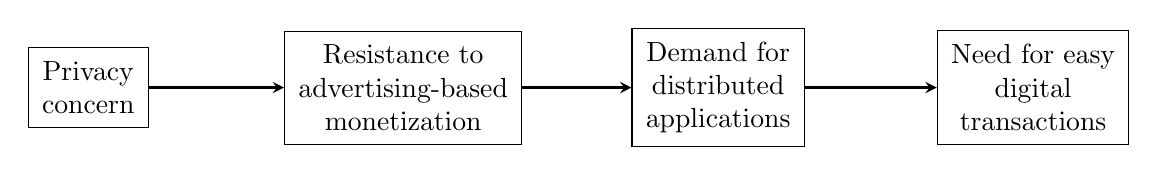
\begin{tikzpicture}[>=stealth]
\node[draw, rectangle, align=center, inner sep=5pt] (p) at (0,0) {Privacy\\concern};
\node[draw, rectangle, align=center, inner sep=5pt] (a) at (4,0) {Resistance to\\advertising-based\\monetization};
\node[draw, rectangle, align=center, inner sep=5pt] (d) at (8,0) {Demand for\\distributed\\applications};
\node[draw, rectangle, align=center, inner sep=5pt] (t) at (12,0) {Need for easy\\digital\\transactions};
\draw[->, thick] (p) -- (a);
\draw[->, thick] (a) -- (d);
\draw[->, thick] (d) -- (t);
\end{tikzpicture}
\caption{An editorial schematic of the Web3 motivation as it is presented in the interview.}
\end{figure}

A careful note must preserve the modesty of the claim. The interview does not provide detailed blockchain architecture, token economics, or cryptographic formalism. It provides a social and commercial motivation: privacy pressure, dissatisfaction with ad-based platforms, distributed interaction, and payment rails that do not always pass through traditional centralized channels.

\section{Cybersecurity as Structural Demand}

From Web3 the interview moves naturally into vulnerability. The interviewer points to recent hacks and asks how important cybersecurity will become over the next ten to twenty years. Glenn's response is immediate and emphatic: massive, massive. He goes so far as to say that if someone wants a highly reliable career entry point in technology, he tells them to consider cybersecurity or information security.

\begin{definition}
In the language of this chapter, the \emph{attack surface} is the effective digital exposure created by interconnection, remote access, cloud dependence, and insecure design choices.
\end{definition}

The spoken logic is straightforward:
\begin{equation}
\text{cloud interconnection} + \text{weak security design}
\Longrightarrow A_{\mathrm{attack\ surface}}\uparrow
\Longrightarrow D_{\mathrm{security\ labor}}\uparrow.
\end{equation}

This is not merely a statement about criminals becoming cleverer. It is a statement about the structure of the systems we build. Glenn says that security is only now entering the mindset of executives and product builders from the design stage onward. His analogy is memorable: we built the digital world as though we were constructing buildings without adequate locks and doors, and then acted surprised when intruders appeared.

\paragraph{Anecdote.} He grounds this claim historically. Early in his career he worked in information security and trained agencies such as the FBI, the CIA, and the IRS. These institutions were used to cases built from file cabinets full of documents. Then the cabinets disappeared and the evidence moved into computers. The immediate problem became forensic science: how to recover deleted documents, how to extract information from machines, how to think about evidence in digital form.

\paragraph{Claim.} Security demand grows because digitization changes not just the medium of work but the medium of failure.

\paragraph{Mechanism.} As information migrates into machines, then into networks, then into cloud-based and highly interconnected systems, compromise becomes both easier and more consequential. The market for security expertise therefore grows structurally rather than cyclically.

\begin{figure}[h]
\centering

\begin{tikzpicture}[>=stealth]
\node[draw, rectangle, align=center, inner sep=5pt] (f) at (0,0) {File cabinets\\and paper records};
\node[draw, rectangle, align=center, inner sep=5pt] (c) at (4,0) {Computers as\\evidence stores};
\node[draw, rectangle, align=center, inner sep=5pt] (r) at (8,0) {Forensic recovery\\of digital data};
\node[draw, rectangle, align=center, inner sep=5pt] (n) at (12,0) {Cloud and network\\interconnection};
\node[draw, rectangle, align=center, inner sep=5pt] (s) at (16,0) {Security by design\\as permanent demand};
\draw[->, thick] (f) -- (c);
\draw[->, thick] (c) -- (r);
\draw[->, thick] (r) -- (n);
\draw[->, thick] (n) -- (s);
\end{tikzpicture}
\caption{An editorial schematic of the security narrative: digitization changes evidence, exposure, and therefore labor demand.}
\end{figure}

The interview gives no formal security model, and we should not invent one. But it does give a very strong causal chain, and that chain deserves to survive intact.

\section{Founder Filters, Time Scarcity, and Recession Deployment}

After the technical middle, the interview returns to the practical question of what it means to build. Glenn says that ideas are easy and doing is hard. He often investigates possible businesses by asking first whether they are viable and second whether, if they succeed, he would actually want to live inside them for years.

\begin{equation}
T_{\mathrm{build}} \gtrsim 3\text{--}5\ \mathrm{years}.
\end{equation}

That timescale is one of the chapter's hardest quantitative constraints. Even successful companies usually require years, and that means the selection problem cannot be reduced to novelty alone.

\begin{itemize}
\item Is the idea viable?
\item If it succeeds, do we want to spend years inhabiting it?
\end{itemize}

The second question is crucial. A business is not merely an exit option. It is a durable environment in which one must work daily. That is why Glenn compares founding, in effect, to creating something that will demand long-term care.

The lecture then becomes even more concrete. He is asked about work-life balance and about the biggest challenge in a first company. The answer is blunt: there were not enough hours in the day. Young children, employees waiting outside the office, family demands, product demands, and administrative demands all compete for the same finite resource.

\begin{equation}
H_{\mathrm{family}} + H_{\mathrm{team}} + H_{\mathrm{product}} + H_{\mathrm{admin}}
= H_{\mathrm{available}}.
\end{equation}

The point is not that he sat down and wrote this equation. The point is that his anecdote about people lined up outside the office, together with children at home and a spouse calling for help, is exactly a conservation law of attention. The founder's day is fixed; the claims on it are not.

There is then a brief but important reinforcement of the cybersecurity thesis. When asked what industry young people should explore for a strong career, he again names information security. The interview thus loops back and confirms that the earlier technology discussion was not just commentary. It was also advice about where durable demand is likely to persist.

\subsection{Question \& Answer}

\paragraph{Question.} What should one do with limited capital in a weak economy?

\paragraph{Answer.} Glenn's answer is conservative in the best sense. With only about \$100{,}000 of initial capital, one should not pretend to have the balance sheet of a heavily funded deep-tech startup. One should either begin with a service business that generates cash flow or, if the technical skill exists, invest labor directly and build the first version oneself.

\begin{equation}
C_{0} \approx 10^{5}\ \mathrm{USD}
\Longrightarrow \text{service revenue first or founder-built product.}
\end{equation}

This is the place where a simple worked example helps. Suppose a founder has fixed deployable capital \(K\) and faces a unit labor cost \(c_{\mathrm{labor}}\). Then the amount of labor input that can be purchased is
\begin{equation}
Q_{\mathrm{labor}}=\frac{K}{c_{\mathrm{labor}}}.
\end{equation}
If recession reduces unit cost from \(c_{1}\) to \(c_{2}\), with \(c_{2}<c_{1}\), then
\begin{align}
Q'_{\mathrm{labor}}-Q_{\mathrm{labor}}
&= \frac{K}{c_{2}}-\frac{K}{c_{1}} \\
&= K\left(\frac{1}{c_{2}}-\frac{1}{c_{1}}\right) > 0.
\end{align}

This is the clean mathematical version of a point Glenn makes several times in prose. Recession is painful, but it is also a repricing event. If labor becomes cheaper, if certain services become cheaper, or if remodeling and other expenditures can be done for less, then the same capital buys more. That is why he does not speak of downturns only in tones of fear. He insists that they are temporary and that, for those with savings and patience, they can create windows for deployment.

We should also preserve the caution in his macroeconomic remarks. His diagnosis of inflation includes the pandemic, supply-chain disruption, and corporate greed. Those are his claims, not settled laws. The durable practical point is narrower: do not imagine that the current bad state of the economy is permanent.

The chapter closes this advisory movement with one more decision rule:
\begin{equation}
\text{domain depth}\uparrow \Longrightarrow \text{decision quality}\uparrow.
\end{equation}
The language around it is simple: stick to what you know, or learn one field deeply enough that your judgment is not second-hand. Do not shotgun capital or attention across whatever happens to be exciting at the moment.

\section{Summary}

The interview begins with a spectacular number and ends somewhere more useful. We start with a billion-dollar sale, but the lasting mathematics of the chapter lies elsewhere: finite hours, multi-year build times, fixed capital, changing input costs, increasing attack surface, and the causal relation between privacy pressure and distributed digital systems. Glenn's lesson is not that one large exit solves life. It is that skill, attention, domain depth, and timing continue to govern action long after the exit has occurred. In that sense the chapter is not really about wealth display at all. It is about disciplined movement inside changing constraints.